\documentclass[11pt]{article}
\usepackage{import}
\usepackage[margin=1in, top=1in]{geometry}
\usepackage[all]{nowidow}
\usepackage[hyperfigures=true, hidelinks, pdfhighlight=/N]{hyperref}
\usepackage[separate-uncertainty=true, group-digits=false]{siunitx}
\usepackage{graphicx,amsmath,physics,tabto,float,amssymb,pgfplots,verbatim,tcolorbox}
\usepackage{listings,xcolor,subfig,caption,import,wrapfig,lipsum,tikz,biblatex}
\usepackage[version=4]{mhchem}
\usepackage[noabbrev]{cleveref}
\newcommand{\creflastconjunction}{, and\nobreakspace}
\newcommand{\mb}[1]{\mathbf{#1}}
\numberwithin{equation}{section}
\numberwithin{figure}{section}
\numberwithin{table}{section}
\definecolor{stringcolor}{HTML}{C792EA}
\definecolor{codeblue}{HTML}{2162DB}
\definecolor{commentcolor}{HTML}{4A6E46}
\captionsetup{font=small, belowskip=0pt}
\lstdefinestyle{appendix}{
    basicstyle=\ttfamily\footnotesize,commentstyle=\color{commentcolor},keywordstyle=\color{codeblue},
    stringstyle=\color{stringcolor},showstringspaces=false,numbers=left,upquote=true,captionpos=t,
    abovecaptionskip=12pt,belowcaptionskip=12pt,language=Python,breaklines=true,frame=single}
\lstdefinestyle{inline}{
    basicstyle=\ttfamily\footnotesize,commentstyle=\color{commentcolor},keywordstyle=\color{codeblue},
    stringstyle=\color{stringcolor},showstringspaces=false,numbers=left,upquote=true,frame=tb,
    captionpos=b,language=Python}
\renewcommand{\lstlistingname}{Appendix}
\pgfplotsset{compat=1.17}
\addbibresource{bibliography.bib}

\begin{document}
    

\section{Background}
The ALICE detector (A Large Ion Collider Experiment) is a detector experiment at the Large Hadron Collider (LHC) at CERN. Its primary goal is the investigation of ``strongly interacting matter at extreme energy densities, where a formation of a new phase of matter, the quark-gluon plasma, is expected'' \cite{ALICE_LOI}. It achieves this goal by studying the products of head-on collisions of heavy ions such as lead, called Pb-Pb collisions for short. It also studies proton-lead (p-Pb) and proton-proton (p-p) collisions.  

% ALICE is situated at 

% The LHC at CERN in Geneva is built to accelerate particles up to very high energies (\SI{13.6}{\tera\electronvolt})

\subsection{Coordinates}
The coordinate system used at ALICE needs to be discussed in order to fully explain the scope of this report. A modified cylindrical coordinate system, shown in \cref{fig:coords}, is used as most detectors in the experiment are cylindrically symmetric about the beamline of the LHC. 

\begin{figure}[h]
    \begin{center}
        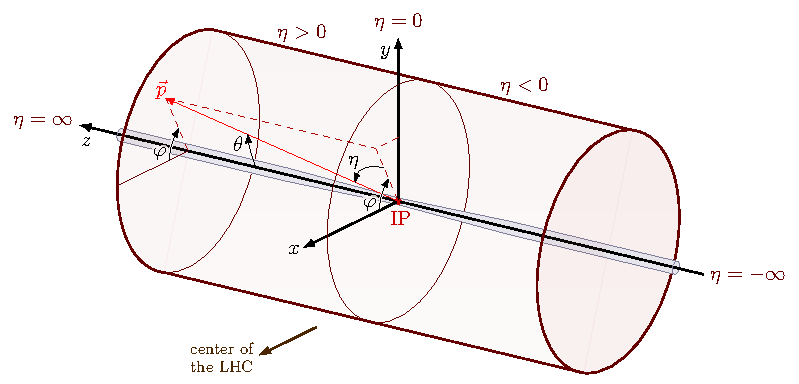
\includegraphics[width=.8\textwidth]{Figs/coords.pdf}
        \caption{Modified cylindrical coordinate system used at the LHC \cite{coords}}
        \label{fig:coords}
    \end{center}
\end{figure}

We place the $z$-axis along the beamline with its origin at the interaction point (IP). The IP is the point at which collisions happen, right in the center of the detector. The angle around the $z$-axis is called the azimuthal angle, denoted by $\varphi$. Sometimes $\phi$ ranges from 0 to $2\pi$, and sometimes it ranges from $-\pi$ to $\pi$. We will try stay consistent and use the latter in this report, but we may need use the other convention at times. The angle from the $z$-axis to the $x-y$ plane is called the polar angle, denoted by $\theta$. $\theta$ runs from 0 to $\pi$. We are interested in the standard 3-momentum of particles that we track in the detector, which we call $\vec{p}=(p_x,p_y,p_z)$, but we also define the transverse momentum as 
\begin{equation}
    p_{\mathrm{T}}=\sqrt{p_x^2 + p_y^2}.
    \label{eqn:transverse momentum}
\end{equation}
We define the rapidity, often denoted as $y$, as
\begin{equation}
    y=\frac 12 \ln\left(\frac{E+p_z}{E-p_z}\right)
    \label{eqn:rapidity}
\end{equation}
where $E$ is the total energy of the particle being considered and $p_z$ is the momentum in the $z$ direction \cite{kar_exp_phys}. This quantity is useful as differences in rapidity are Lorentz invariant for boosts along the $z$-axis. One issue, however, is that the energy of a particle is hard to measure, so we instead use pseudorapidity, denoted as $\eta$. Rapidity and pseudorapidity are equivalent for massless particles, and near equivalent for particles with total 3-momentum magnitude $p$ much greater than their mass $m$. Pseudorapidity is much easier to measure as it is defined as \cite{kar_exp_phys}
\begin{equation}
    \eta=-\ln\tan\frac{\theta}{2}.
    \label{eqn:pseudorapidity}
\end{equation}
From \cref{fig:coords} we see that for $z$ positive, $\eta$ is also positive, and similarly for $z$ negative. Confusingly, we define the ``forward region'' of the ALICE detector as the region for which $z$, and thus $\eta$, are negative. 

\subsection{ALICE Run 3}
In 2018, the LHC shut down for what was called Long Shutdown 2 (LS2). During this time, the ALICE experiment was being prepared for what is called Run 3, where it will be taking data at much higher rates and much higher energies than before \cite{ALICE_Upgrade_LOI}. \Cref{fig:ALICE_Schematic} shows the detector configuration for Run 3. The intent of these upgrades was in large part to prepare ALICE for higher frequency collisions in both Pb-Pb and p-p cases. 

\begin{figure}[h]
    \begin{center}
        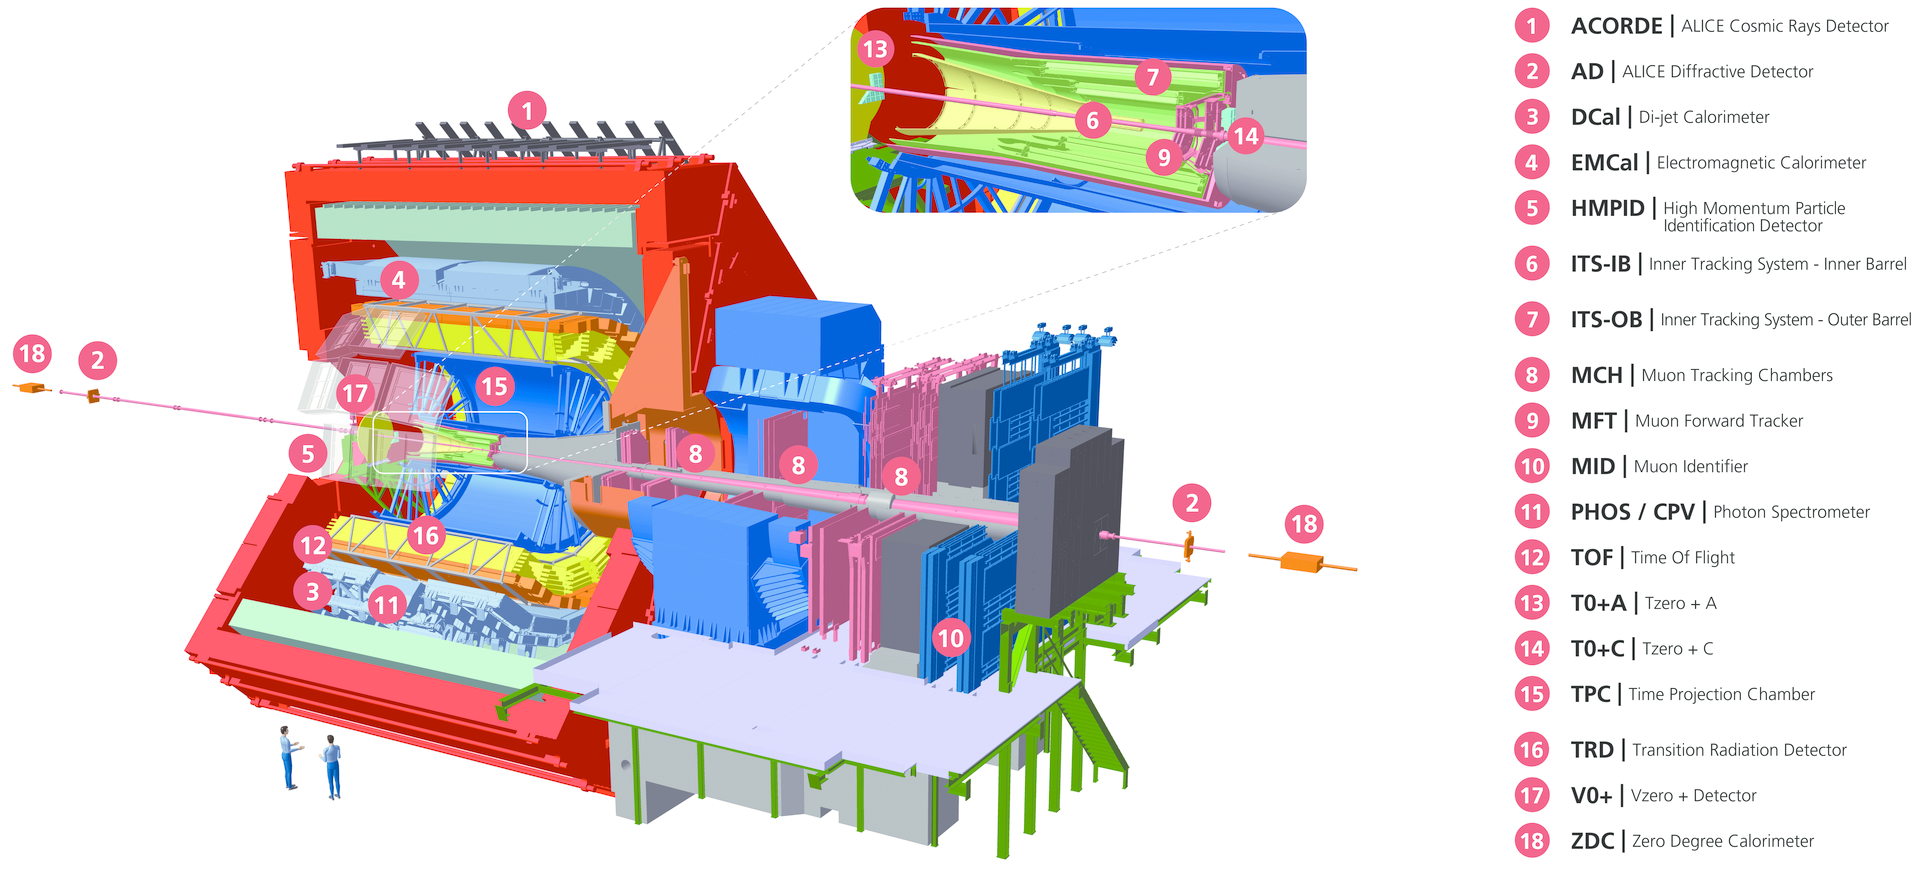
\includegraphics[width=.8\textwidth]{Figs/ALICE_RUN3_schematic.png}
        \caption{ALICE Run 3 schematic}
        \label{fig:ALICE_Schematic}
    \end{center}
\end{figure}

Part of the upgrades for Run 3, the details of which can be found in \cite{ALICE_Upgrade_LOI}, were a whole new Inner Tracking System (ITS) and a brand new detector called the Muon Forward Tracker (MFT). These detectors are both silicon-based and their primary purpose is tracking particles. 

The readout electronics for many detectors were also upgraded to allow for continuous readout as opposed to triggered readout. The MFT, however, will still work on a triggered readout system as \textit{\textbf{I THINK BECAUSE EVENTS ARE LESS COMMON DUE TO THE ABSORBER BUT IDK FOR SURE}}.

\subsection{The Muon Spectrometer}
The Muon Spectrometer (\textit{\textbf{MCH or MUON, not sure}}) sits in the forward region of ALICE, as seen in \cref{fig:ALICE_Schematic}. It is designed to study heavy quark resonances through their single- and di-muon decay channels

As is shown in \cref{fig:Muon Spectrometer}, it is composed of an absorber, tracking chambers, a dipole magnet, and finally the trigger chambers, often called the Muon Identifying Detector (MID) [maybe]. The MFT is also considered part of the MCH but is not shown in \cref{fig:Muon Spectrometer}. The absorber serves to filter out all particles travelling towards the MCH that are not muons as muons interact very rarely with matter. The 5 tracking chambers track the path of the muons before, during, and after they are bent by the dipole magnet. These tracking chambers used to do the job of the MFT in Run 1 and Run 2, but with the increase in luminosity and energy of the LHC in Run 3, the MFT needed to be added in order to vastly improve the vertexing capabilities. Lastly, the trigger system is made of two large gas chamber detectors. 

\begin{figure}[h]
    \begin{center}
        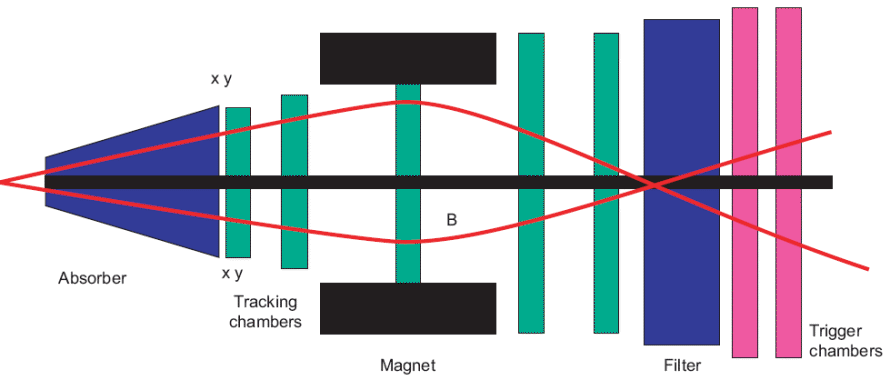
\includegraphics[width=.8\textwidth]{Figs/MCH_schematic.png}
        \caption{Muon Spectrometer Diagram}
        \label{fig:Muon Spectrometer}
    \end{center}
\end{figure}








\subsection{The Muon Forward Tracker}
The MFT is a brand new detector added to ALICE for Run 3. It serves as a tracking detector for the Muon Spectrometer (\textit{\textbf{MCH or MUON, not sure}}), which sits in the forward region ($-4<\eta<-2.5$). The MFT was made in conjunction with the ITS and uses precisely the same silicon CMOS sensors but in a different configuration to better suit the geometry of the problem. At its closest point, the MFT is only \SI{46.0}{\milli\metre} from the IP, and \SI{76.8}{\centi\metre} at its furthest. 



\subsection{The Inner Tracking System}




\subsection{The Online-Offline Analysis Framework (O2)}

\printbibliography

\end{document}
